\documentclass[twocolumn]{paper}

\usepackage[width = 17cm]{geometry}
\usepackage{tikz}
\usetikzlibrary{arrows.meta, positioning}
\usepackage{graphicx}
\usepackage{subcaption}
\usepackage{amsmath}
\usepackage{amssymb}
\usepackage{amsfonts}
\usepackage{braket}
\usepackage[english]{babel}
\usepackage{natbib}
\setcitestyle{numbers}
\setcitestyle{square}
\usepackage{hyperref}
\usepackage{xcolor}

\newcommand{\incfig}[1]{%
    \def\svgwidth{\columnwidth}
    \import{./figures/}{#1.pdf_tex}
}

\newcommand{\marginnote}[1]{\textsuperscript{*}\marginpar{\fbox{\parbox{2cm}{\textcolor{blue}{#1}}}}}


\title{Revisiting semiclassical scalar QED in 1+1 dimensions }
\author{Authors}


\begin{document}
\makeatletter
\maketitle

\begin{abstract}
In this article we study the backreaction of a charged quantum scalar field on a background classical constant electric field in a finite one-dimensional region, with attention to boundary effects. We review previous work in this setup \cite{ambjorn_properties_1983}, where it was found that vacuum polarization averts instabilities due to runaway solutions. Their prescription for computing the vacuum polarization was later pointed out to be incorrect \cite{schlemmer_current_2015}, and a correct, gauge-invariant definition using Hadamard point-splitting was introduced \cite{wernersson_vacuum_2021}, yielding a vacuum polarization an order of magnitude weaker. Applying this correct prescription through an iterative procedure across varying boundary conditions and masses, we find that the system remains stable despite the weaker vacuum polarization. Interestingly, the numerical discrepancies between the two prescriptions do not extend to the strong-field regime, where their behavior is remarkably similar; we attribute this to the dominant low-energy modes being the most sensitive to the background field.
\end{abstract}

\tableofcontents

\section{Introduction}



Vacuum polarization is a phenomenon in quantum electrodynamics (QED) by which the vacuum of a charged field polarizes when subject to external electric fields, effectively behaving like a dielectric with $\epsilon>0$. This mechanism was one of the first QED effects studied \cite{dirac_discussion_1934}, with consequences that followed closely \cite{uehling_polarization_1935,heisenberg_consequences_1936}. This mechanism has been already observed, e.g.~in corrections to atomic levels \cite{lamb_fine_1947} (cf. Ref.~\cite{mohr_qed_1998} for a review), while others e.g.~the Schwinger effect \cite{schwinger_gauge_1951} lay beyond current technological advances (cf. Ref.~\cite{fedotov_advances_2023}). 
Particularly, interest in the Schwinger model has seen an increase in the context of lattice gauge theory, as it is one of the simplest models of a gauge theory that one can simulate, thus becoming a playground for testing novel analytical and numerical methods \cite{banuls_mass_2013,banuls_thermal_2015}. 

Defining vacuum polarization  for general backgrounds\footnote{ And other observables relying on the evaluation of products of fields at coinciding points.} is no easy task. Historically, \cite{dirac_discussion_1934} first defined it by assuming that the short-distance behavior of a class of states when background electric fields are present is the same, modulo smooth coefficients, as in the no background field case. In modern bibliography, these states are called Hadamard, see e.g.~\cite{fewster_necessity_2013}, and are particularly interesting in the context of quantum field theory on curved spacetimes, where the same idea is used to define observables necessary for the study of e.g.~perturbative interacting field theory or semi-classical gravity (cf.~\cite{hollands_quantum_2015,hollands_local_2001} for detailed discussions on the definition on such observables).

Semi-classical gravity, a possible first step towards a quantum theory of gravity, couples classical gravity  to the expectation value of the stress-energy tensor, which as stated above needs to be properly defined. To our knowledge, only perturbative corrections to the metric have been studied  \cite{thompson_quantum-corrected_2024}. In this article we study, as a toy model, the effect of the backreaction of a charged scalar field to a background classical electric field in 1+1 dimensional Minkowski spacetime. This setup was already studied in  \cite{ambjorn_properties_1983}, where it was found that ignoring the backreaction of the scalar field leads to instabilities, and it is claimed that its inclusion avoids them.
However, as pointed out in \cite{schlemmer_current_2015}, the expression for $\rho$ used in \cite{ambjorn_properties_1983} cannot be derived from a gauge invariant prescription. Thus, the question arises: Does using the correct renormalization prescription also avoid these instabilities? We will use the prescription described in \cite{wernersson_vacuum_2021} to implement an iterative method to study the effect of the backreaction of the scalar field. It has been found that this expression also alleviates the above mentioned instabilities.  

The layout of this article is as follows: Section 2 ...

\textbf{Maybe add?}: \cite{costeri_hadamard_2025} discusses hadamard states in the pressence of time-like boundaries.

This article summarizes and extends the results of the M.Sc. thesis of Santiago Sanz-Wuhl, written in 2025 at the Institut für Theoretische Physik, Universität Leipzig, under the supervision of Jochen Zahn.
\section{Set up} 

1+1 dimensional spacetime, two charges $q, -q$
are set at $x^1=0, x^{1}=a$, respectively. Ignoring vacuum polarization effects,
this yields a constant electric field of strength $q$ pointing towards positive $x^{1}$.
We study the solutions to the semiclassical Klein-Gordon-Maxwell equations
\begin{subequations}
    \begin{align}
        \left( D_\mu D^\mu + m^2 \right)\phi &= 0, \\
        \label{eq:KG}
        \partial_\mu F^{\mu\nu} &= \left< j^\nu \right>_\Omega,
        \label{eq:Maxwell}
    \end{align}
\end{subequations} in the region $x \in     \mathbb{R} \times [0,
a]$. Here, $D_\mu = \partial_\mu +ie A_\mu$ defines the gauge covariant
derivative, \begin{align}
    j^\nu = \frac{ie}{2} \left((D^\nu \phi^*) \phi - \phi^*
    D^\nu \phi \right)
\end{align}
is the charge current density of the Klein-Gordon field, and
$\left< \right>_{\Omega}$ takes its expectation value with
the scalar field in the state $\Omega.$ 
The solutions looked for are the Maxwell tensor $F^{\mu
\nu}$ and the two-point function of the vacuum state $\Omega$. Following
\cite[]{Ambjorn:1981xv, Wernersson:2020xeh}, the metric signature
is $(+,-)$.

In choosing the Coulomb gauge $\partial_1 A_1=  0$, the spatial component
of $A_\mu$ will in general be a constant that is gauged away to 0. Setting $\nu =0$ in Eq.~\eqref{eq:Maxwell} yields the Poisson equation for the electrostatic potential $A_0$
\begin{align}
    \partial_1^2 A_0(x^1) =  -\rho, \label{eq:poisson}
\end{align} 
with 
\begin{align}
    \rho =  \left< j^0 \right>_0 = \frac{ie}{2} \bra{0} (\partial_1
    \phi^*) \phi -\phi^* \partial_1 \phi \ket{0}
\end{align}
the vacuum polarization, i.e. the vacuum expectation value (VEV)\marginnote{In case the words VEV turn up again.} of the zeroth component of the charge current density. $\ket{0}$ is the vacuum state of the scalar field. 
Eq. \eqref{eq:poisson} will be solved with the boundary conditions
\begin{align}
    \left. \partial_1
        A_0(x^1)\right|_{x^1=0, a} =  -q
        \label{eq:A0-boundary-conditions}
\end{align}
so that a measurement of the electric
field close to the boundary is not screened by the vacuum polarization.
This fixes the solution to Eq.~\eqref{eq:poisson} up to an addition constant,
which is conveniently chosen so that $A_0(\frac{a}{2}) = 0$. For a given charge
density $\rho(x^{1})$, Eq.~\eqref{eq:poisson} is solved by
\begin{align}
        A_0(x^1) = -q\left(x^1 - \frac{a}{2} \right) -
        \int_{\frac{a}{2}}^{x^{1}} \int_{0}^{\chi} \rho(\xi) d \xi d \chi.
    \label{eq:A0-general} 
\end{align}


\section{Field modes}

In the chosen gauge, the Klein-Gordon equation is of the form \begin{align}
    \left[ (\partial_0 + ie A_0 )^2 + \partial_1^2 - m^2
    \right]\phi = 0,
    \label{eq:TDKGE}
\end{align}
which will be studied using different boundary conditions. We will consider Dirichlet  $\left.\phi \right|_{x^{1}=0,a} = 0$ and Neumman $\left.\partial_{1} \phi\right|_{x^1=0,a }=0$ boundary conditions, although more general Robin boundary conditions may be considered.

With the single frequency ansatz $\phi_n(x) = \phi_n (x^{1}) e^{-i\Omega_n x^0}$,
Eq.~\eqref{eq:TDKGE} is split into ordinary differential equations for each 
of the modes
\begin{align}
    \left[ (\Omega_n - e A_0 )^2 + \partial_{1}^2 -  m^2 \right]\phi_n
    = 0,
    \label{eq:TIKGE}
\end{align}
where the frequencies $\Omega_n$ are gauge dependent and to be determined by
the boundary conditions.

Following \cite{Ambjorn:1981xv}, the following dimensionless parameters
are defined 
\begin{itemize}
    \item $z = \frac{Z}{a}$,
    \item $\lambda = e E a^2,$
    \item $\varepsilon = ea$,
    \item $\omega_{n} = a\Omega_{n, \alpha} + \lambda \alpha$,
\end{itemize}
where $\alpha \in \mathbb{R}$ is a parameter characterizing
global gauge transformations of the form \begin{align}
    \varepsilon A_0 \to \varepsilon A_0 + \lambda\alpha.
\end{align} This way, the mode energies $\omega_n$ are ensured to be gauge invariant,
and Eq.~\eqref{eq:TIKGE} takes the form \begin{align}
    \left[ (\omega_n - \varepsilon A_0 )^2 + \frac{d^2}{dz^2} - a^2
    m^2\right] \phi_n = 0.  \label{eq:mode-equation}
\end{align}
The modes $\phi_n$ are normalized with respect to the symplectic
norm
\begin{align}
    (\phi_n, \phi_m) = i\int_{0}^{1} (\phi_n^* \pi_m^* - \pi_n \phi_m)dz,
\end{align}
with $\pi_n = (D_0 \phi_n)^*$ the canonical conjugate of
$\phi_n$.

The general solution to Eq.~\eqref{eq:TDKGE} is thus decomposed in
modes \begin{align}
    \phi(t, z) = \sum_{n>0}^{} a_n \phi_n(z) e^{-i\omega_n t} +
    \sum_{n<0}^{} b^\dagger_n \phi_n(z) e^{-i\omega_n t},
\end{align} where positive (negative) values of $n$ correspond to modes of positive
(negative) norm. $a_n$ and $b_n$ are the ladder operators for the positive and
negative norm solutions, respectively, obeying the commutation relations
\begin{align*}
    [a_n, a_n^\dagger ] = [b_n, b_n^\dagger ] =\delta_{nm}
\end{align*}
and all other commutators vanishing. The ladder operators define
the vacuum state $\ket{0}$ as that for which $a \ket{0} = b\ket{0} = 0$.
As it is above mentioned, the definition of operators such as the vacuum
polarization is problematic, since it involves the product of local observables 
evaluated at coinciding spacetime points. 

The definition of such observables is done by point-splitting with respect to a
Hadamard parametrix, originally used by Dirac\marginnote{Add
citation}, and further developed in the
context of Quantum Field Theory in Curved Spacetimes (cf. \cite{Wald:1977up}).
Dirac originally defined the vacuum polarization by assuming that the behavior
of the field in the presence of background electromagnetic fields was the same
as that in the absence thereof, modulo smooth coefficients. Today, this
assumption on the short-distance behavior of the fields is called the Hadamard
condition. It is generally accepted that all physically relevant states
$\Omega$ are of this form, where the short-distance divergence structure of the
field is covariant, local, state independenent, and constructed from the
background, i.e. the gauge connection.

Under this condition, the two-point function $w_{\Omega}^{\phi \phi^*} =
\bra{\Omega} \phi(x) \phi^*(x') \ket{\Omega} $ of the scalar field $\phi$ in
the state $\Omega$  acquires the form
\begin{align}
    w_{\Omega}^{\phi\phi^*}(x, x') 
    = H^{\phi \phi^*}(x, x')  + R^{\phi \phi^*}_{\Omega} (x, x').
    \label{eq:hadamard-condition}
\end{align}
Here,
\begin{equation}
    H^{\phi\phi^*} = -\frac{V_0(x,x')}{4\pi} \ln [(t-t')^2 -
    (z-z')^2 + i\varepsilon \sign (t-t')]
    \label{eq:hadamard-parametrix}
\end{equation}
is the Hadamard parametrix of the scalar field in two spacetime dimensions, up
to order relevant for the vacuum polarization, and $R_{\Omega}^{\phi\phi^*}$
is a smooth function. 
\begin{equation}
    V_0(x, x') = \exp\left[-i\varepsilon \int_{0}^{1} A_{\mu}(x' +
    s(x-x') ) (x - x')^{\mu}ds \right]
\end{equation} 
is the parallel transport, which preserves gauge invariance in the coinciding
point limit. The Hadamard condition allows us to define expectation values of
local observables non-linear in the fields:
\begin{align}
    \left< D_\alpha \phi (x) D^{*}_\beta \phi^*(x) \right> = \lim_{x' \to x}
    D_\alpha D^{*}_\beta' (w_\Omega^{\phi \phi^*}(x, x')- H^{\phi\phi^*}(x,
    x')),
    \label{eq:point-splitting}
\end{align}
with $\alpha, \beta$ are symmetrized multiindices.

\begin{figure}[t]
    \begin{subfigure}{0.5\textwidth}
        \centering
        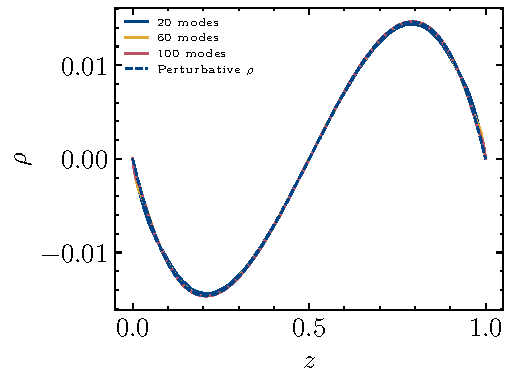
\includegraphics[width=1\textwidth]{Figures/dirichlet/unfilteredRhoaa.pdf}
    \end{subfigure}
    \begin{subfigure}{0.5\textwidth}
        \centering
        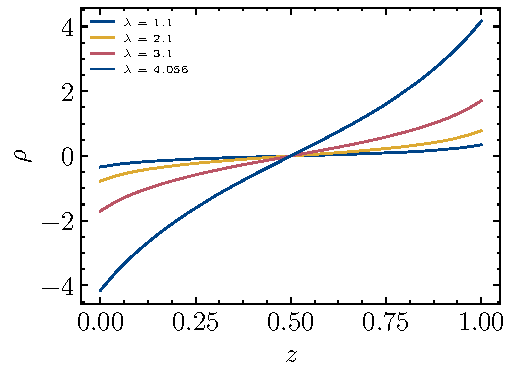
\includegraphics[width=1\textwidth]{Figures/neumann/vacuumPolarizationEvolution.pdf}
    \end{subfigure}
    \caption{The vacuum polarization $\rho$ of the scalar field: In the left
    panel, $m=0$ and using Dirichlet boundary conditions. In the right panel,
    $m=1$ using Neumann boundary conditions.}
    \label{fig:Figures-dirichlet-unfilteredRhoaa-pdf}
\end{figure}

As it was calculated in \cite[]{Wernersson:2020xeh} the vacuum polarization as
defined through point-spliting with respect to $H^{\phi\phi^*}$ yields
\begin{align}
    \rho = \lim_{\tau \to 0} \sum_{n>0}^{} (\omega_n - \varepsilon A_0) \lvert
    \phi_n\rvert^2 e^{-i\omega_n \tau} +\sum_{n<0}^{} (\omega_n - \varepsilon
    A_0) \lvert \phi_n\rvert^2 e^{i\omega_n \tau} + \frac{\varepsilon^2}{\pi}
    A_0 .
    \label{eq:vacuum-polarization-long}
\end{align}
Two examples of $\rho$ calculated using this expression are shown in
Fig.~\ref{fig:Figures-dirichlet-unfilteredRhoaa-pdf}\marginnote{Obviously need
to be redone.}. These are calculated with a constant background electric field
(the external field approximation explained below), with the corresponding mass
and boundary conditions explained in the caption.

To measure the \textit{strength} of the vacuum polarization, the induced charge
\begin{align}
    Q_I = \int_{0}^{\frac{1}{2}} \rho(z) dz
    \label{eq:polarized charge}
\end{align}
is defined. This charge will screen the background electric field $\lambda$,
and Gauß's law yields that the total electric field at $z=\frac{1}{2}$ is
$\lambda + Q_I$.

\subsection{External Field Approximation and critical $\lambda$}
\label{subsec:External-Field-Approximation}

The external field approximation ignores the contribution of the backreaction
of the charged scalar field to the background electric field. This
approximation displays the instabilities of the system, which the inclusion of
backreaction aims to avoid. Thus, Eq.~\eqref{eq:mode-equation} is solved with
$A_0(z) = -\lambda (z - \frac{1}{2})$, and takes the form
\begin{figure}[t]
    \centering
    \begin{subfigure}{0.45\textwidth}
        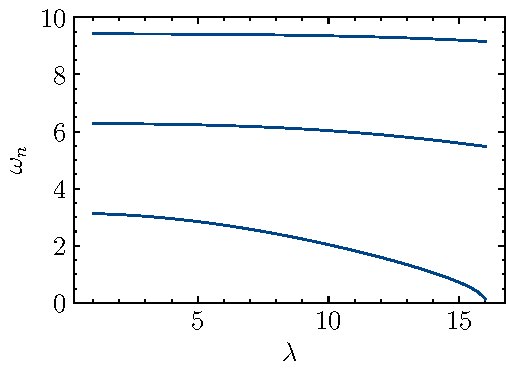
\includegraphics[width=\textwidth]{Figures/dirichlet/eigenvaluesExternalFieldApproximation.pdf}
    \end{subfigure}
    \begin{subfigure}{0.45\textwidth}
        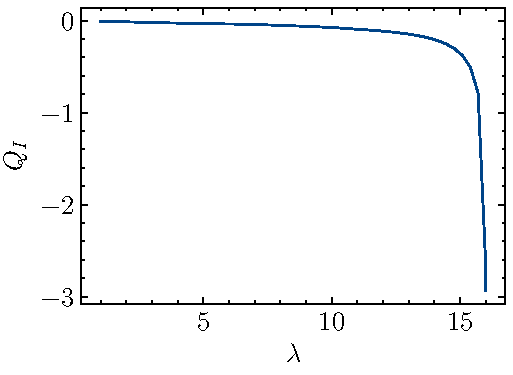
\includegraphics[width=\textwidth]{Figures/dirichlet/inducedChargeExternalFieldApproximation.pdf}
    \end{subfigure}
    \caption{Left panel: Energy of the three first modes of the massless
    Klein-Gordon field with Dirichlet boundary conditions
    corresponding to different values of the dimensionless backgroud
    electric field strength $\lambda.$ Note the apparition
    of $\lambda_c \approx 16.05$ where $\omega_n \to 0.$
Right panel: Corresponding induced charge $Q_I$ as a function of $\lambda$.}
    \label{fig:eigenvalues-external-field-approximation}
\end{figure}
\begin{align}
    \left[ \left(\omega_n + \lambda \left(z-\frac{1}{2}\right) \right)^2 +
    \frac{d {^2}}{d {z^2}} - a^2m^2
\right] \phi_n = 0.  
\label{eq:external-field-approximation-kg}
\end{align}
For each value of $\lambda$, the modes $\phi_n$ and their energies  $\omega_n$ 
can be obtained from the boundary value problem\footnote{The mode solution can 
in fact be written as a linear combination of parabolyc cylinder functions,
as Eq.~\eqref{eq:external-field-approximation-kg} can be rewritten as the Weber equation \cite[]{Ambjorn:1981xv}.}. 
Fig.~\ref{fig:eigenvalues-external-field-approximation} displays the energies
$\omega_n$ of the first three modes $\omega_1, \omega_2, \omega_3$ of the
massless scalar field with Dirichlet boundary conditions as functions of the
background field strength $\lambda$. Notice how the lower curve, corresponding to
$\omega_1$, drops to  $0$ at $\lambda \approx 16$. At that same value of
$\lambda$, the induced charge diverges, as displayed in the left panel of
Fig.~\ref{fig:eigenvalues-external-field-approximation}. This behaviour defines
the critical $\lambda_c$, which adopts different values for different boundary
conditions and masses. As seen in \cite[]{Ambjorn:1981xv}, $\lambda>\lambda_c$
leads to complex mode energies and thus instabilities.

%The modes $\phi_n$ and their
%energies $\omega_n$ can easily be calculated as a boundary
%value problem.	The energies $\omega_n$ of the first three
%modes are displayed for $m=0$ and Dirichlet boundary conditions in
%Fig.~\ref{fig:eigenvalues-external-field-approximation}, as functions of
%the background field strength $\lambda$. The lower curve, corresponding
%to $\omega_1$, drops to  $0$ at $\lambda \approx 16$. This defines
%the critical $\lambda_c$, which appears also for $m\neq 0$ and other
%boundary conditions. As shown by \cite[]{Ambjorn:1981xv}, for values
%$\lambda>\lambda_c$, some frequencies $\omega_n$ turn complex, which
%from the single frequency ansatz leads to runaway solutions.
%
It is claimed in \cite[]{Ambjorn:1981xv}, that the inclusion of
backreaction avoids these instabilities. However, the expression used
for the vacuum polarization is incorrect and one should rather use the
prescription described in \cite[]{Wernersson:2020xeh}. This article
answers the following question: does considering the backreaction
using the correct prescription for the vacuum polarization avoid the
instabilities that would otherwise be present?


%Fig.~\ref{fig:eigenvalues-external-field-approximation} displays the
%energy of the first three modes of the massless Klein-Gordon field with
%Dirichlet boundary conditions\marginnote{Look for a nice abbreviation
%of this. MDBCs? MD KG field?} for different values of $\lambda$ is
%shown. Shows the appearance of $\lambda_c$ as $\omega_n \to 0$, which
%corresponds to $\lambda_c \approx 16$ for this case.



\section{Self-consistent fields}
\label{sec:The-iterative-procedure}

The effect of the backreaction of the scalar field to the background
electromagnetic field is studied by an iterative procedure. 
For each value of $\lambda$, at each iteration $\kappa$, one computes the following
\begin{subequations}
   \label{eq:iterative-procedure}
\begin{align}
    \frac{d {^2}\phi_{n, \lambda}^{\kappa}}{d {z^2}} {}  &= 
    -\left[ (\omega_{n, \lambda}^\kappa - \varepsilon A^{\kappa -1 }_{0, \lambda} )^2 
     - a^2 m^2\right] \phi_{n, \lambda}^{\kappa}, 
    \label{eq:mode-equation-iterative}
    \\
\begin{split}
        \rho_\lambda^{\kappa} &= \lim_{\tau \to 0} \Big[\sum_{n>0}^{} (\omega_{n,
        \lambda}^\kappa - \varepsilon A_{0, \lambda}^{\kappa-1} )\lvert \phi_{n,
        \lambda}^\kappa\rvert^2 e^{-i\omega^\kappa_{n, \lambda} \tau}\\
        &+\sum_{n<0}^{} (\omega^{\kappa}_{n, \lambda} - \varepsilon
        A_{0, \lambda}^{\kappa-1}) \lvert \phi^\kappa_{n, \lambda}\rvert^2
    e^{i\omega^{\kappa}_{n, \lambda} \tau}\Big] \\
    &+
    \frac{\varepsilon^2}{\pi}    A_{0, \lambda}^{\kappa-1} ,
\end{split}
\label{eq:vacuum-polarization-iterative}\\
\begin{split}
        A^{\kappa }_{0, \lambda} &= c A_{0, \lambda}^{\kappa-1} \\&+ \left(1-c
        \right)\left[ -\lambda\left(z - \frac{1}{2} \right) -
            \int_{\frac{1}{2}}^{z} \int_{0}^{\chi} \rho_\lambda^{\kappa}(\xi) d\xi d\chi
             \right] .
\end{split}
        \label{eq:A0-general-iterative}
\end{align}
\end{subequations}
This procedure has two main differences from the one used in \cite{ambjorn_properties_1983}: the expression for the vacuum polarization, and the $c<1$ prescription in Eq.~\eqref{eq:A0-general-iterative}.
The details on how $\rho$ is calculated are explained in Appendix~\ref{sec:Computing-the-vacuum-polarization}. Initial conditions of this procedure are discussed below.

Noticing how Eq.~\eqref{eq:A0-general-iterative} acts as an update function  on $A_{0,\lambda}^{\kappa-1}$, we write this scheme as an infinite dimensional fixed point problem. This is, for each $\lambda$, we look for the fixed point $A_{0, \lambda}$ obeying
\begin{align}
    A_{0, \lambda} = f_\lambda(A_{0, \lambda}),
    \label{eq:fixed-point-problem}
\end{align}
with $f_\lambda$ given by the composition of steps \eqref{eq:mode-equation-iterative}, \eqref{eq:vacuum-polarization-iterative} and \eqref{eq:A0-general-iterative}. 
The fixed points of $f_\lambda$, denominated ``self-consistent solutions", are looked for by studying the limit $A_{0,\lambda}=\lim_{\kappa\to \infty}A_{0,\lambda}^{\kappa}$, where 
\begin{align}
    A_{0,\lambda}^{\kappa + 1} = f_\lambda(A_{0,\lambda}^{\kappa}) =
    f_\lambda^{\kappa}\left(A_{0, \lambda}^{0} \right), \textrm{with } f_\lambda^\kappa =
    \underbrace{f_\lambda \circ ... \circ f_\lambda}_{k \textrm{ times}}.
    \label{eq:self-consistent-limit}
\end{align}
If the limit $A_{0, \lambda}$ exists, it is given the name
self-consistent potential, as well as the corresponding self-consistent vacuum
polarization $\rho_{\lambda}$, field modes $\phi_{n,
\lambda}$ and mode energies $\omega_{n, \lambda}$.

For low enough $\lambda\ll \lambda_c$, the initial value of the sequence $A_{0,
\lambda}^0$  can be set to the external field approximation $A_{0,
\lambda}^0(z) = -\lambda \left(z- \frac{1}{2}\right).$ This is, however,  no longer a valid initial potential for stronger background fields,  as it leads to non-convergences in the sequence $ A_{0, \lambda}^{\kappa}$. This is discussed in the Appendix ??(to be added). For higher $\lambda$-values,
$A_{0, \lambda}^{0}$ is instead set by a stored previously calculated self-consistent
potential $A_{0, \lambda'}$ with $\lambda = \lambda' + \Delta
\lambda$, where $\Delta \lambda > 0$. We use this scheme to probe the $\lambda$-parameter space.



Finally, in Eq.~\eqref{eq:A0-general-iterative}, $c\in [0, 1]$ is introduced in order to ``relax" the procedure: For
$c=0$, the procedure is precisely the one used in~\cite[]{ambjorn_properties_1983}, and it is expected to quickly converge. For
$c$ close to 1, updates will be small corrections to the previous potential.
%This avoids certain numerical instabilities appearing in the strong-field regime $\lambda \gtrsim \lambda_c$. 
Stronger background field strengths increase the instability of the coupled system, thus increasing the relevance of slower converge schemes. 
Considering this, we adopt a scheme in which, as $\lambda$ increases, $c$ increases and simultaneously $\Delta \lambda$ decreases.

%The mode subindices have been removed to avoid notation clutter.
%The iterative procedure is schematized in Fig.~\ref{fig:iterative-procedure},
%and it studies $\lim_{\kappa \to \infty} A_\lambda^\kappa $ for each $\lambda$.
%If the limit exists, it defines the self-consistent potential
%$A^{\infty}_\lambda$. Additionally, every other relevant quantity
%$\rho^\infty_\lambda, \omega_\lambda^{\infty}, \text{ and } \phi_\lambda
%^{\infty}$ also acquire the adjective ``self-consistent".

\begin{figure}[t]
\begin{center}
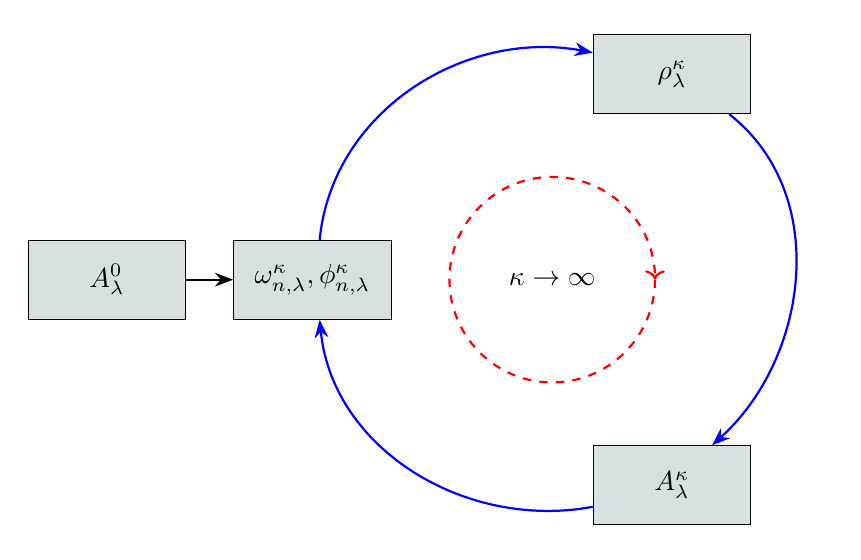
\begin{tikzpicture}[
    scale=0.87,
    box/.style = {draw, rectangle, minimum width=2cm, minimum height=1cm, fill={rgb:red,1;green,2;blue,2}, fill opacity=0.2, text opacity = 1},
    arrow/.style = {->, thick, >=Stealth},
    curved arrow/.style = {->, thick, >=Stealth, bend left}
]
% Nodes
\node[box] (A0) at (0, 0) {$A_{\lambda}^{0}$};
\node[box] (phi) at (3, 0) {$\omega_{n, \lambda}^\kappa, \phi_{n, \lambda}^\kappa$};
\node[box] (rho) at (8.25, 3) {$\rho_\lambda^\kappa$};
\node[box] (tildeA0) at (8.25, -3) {$A_\lambda^{\kappa}$};
\node (kappa) at (6.5, 0) {$\kappa \to \infty$};

% Arrows
\draw[arrow] (A0) -- (phi);

\draw[curved arrow, blue] (phi) to[out=50, in=135] (rho);
\draw[curved arrow, blue] (rho) to[out=55, in=135] (tildeA0);
\draw[curved arrow, blue] (tildeA0) to[out=45, in=130] (phi);

  %\draw[arrow] (phi) to[out=70, in=150, looseness=1] (rho);


% Central evolution arrow
\draw[->, thick, dashed, red] (8, 0) arc[start angle=360, end angle=0, radius=1.5cm];
%\draw[->, thick, dashed, red] (10, 0) arc[start angle=0, end angle=360, radius=3.5cm];

\end{tikzpicture}
\end{center}
\caption{Schematic of the iterative procedure.}%
\label{fig:iterative-procedure}
\end{figure}




%For a low $\lambda\ll \lambda_c$, the initial potential $A_\lambda^{0} = -\lambda
%\left(z-\frac{1}{2}\right)$ is given by the external field approximation. For
%higher values of $\lambda$, $A_\lambda^{0}$ is given by an already calculated
%self-consistent $A_{\lambda'}^{\infty}$, with $\lambda = \lambda' + \Delta
%\lambda$, for $\Delta \lambda > 0 $. 

\section{Results}%
\label{sec:Results}

\begin{figure}[p]
    \centering
    \begin{subfigure}{0.45\textwidth}
        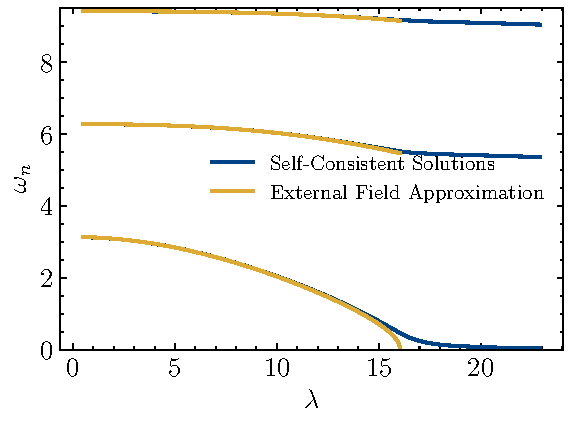
\includegraphics[width=\textwidth]{Figures/dirichlet/eigenvalues.pdf}
    \end{subfigure}
    \begin{subfigure}{0.45\textwidth}
        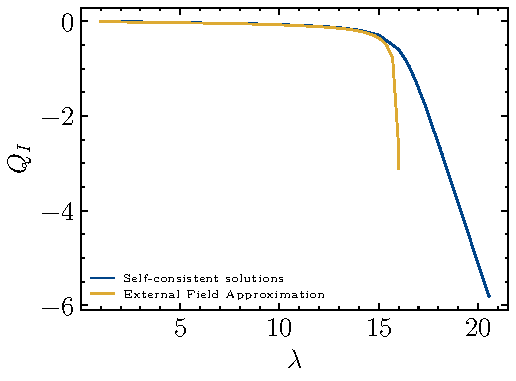
\includegraphics[width=\textwidth]{Figures/dirichlet/inducedCharge.pdf}
    \end{subfigure}
    \begin{subfigure}{0.45\textwidth}
        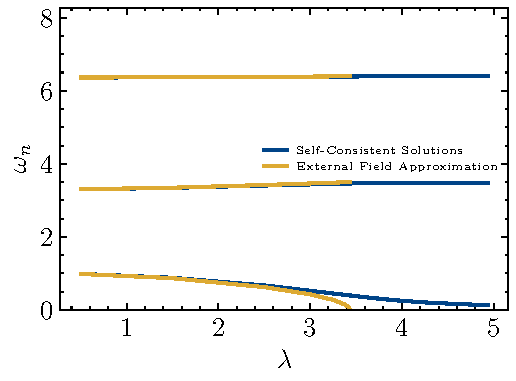
\includegraphics[width=\textwidth]{Figures/neumann/eigenvalues.pdf}
    \end{subfigure}
    \begin{subfigure}{0.45\textwidth}
        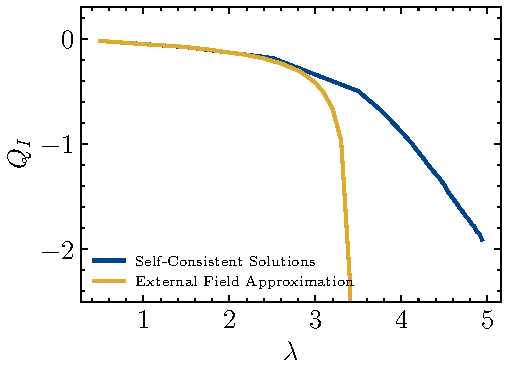
\includegraphics[width=\textwidth]{Figures/neumann/inducedCharge.pdf}
    \end{subfigure}
    \caption{Top left panel: Energy of the three first modes of the massless
    Klein-Gordon field with Dirichlet boundary conditions
    corresponding to different values of the dimensionless backgroud electric
    field strength $\lambda.$ In blue, the self-consistent mode energies
    $\omega_{n,\lambda}^{\infty}$. For reference, the energies of the lower
    modes in the External Field Approximation is shown. Top right panel:
    Corresponding induced charge $Q_I$ as a function of $\lambda$.
    Bottom left panel:
    Massive $(m=1)$ Klein-Gordon field with Neumann boundary conditions
    corresponding to different values of the dimensionless backgroud
    electric field strength $\lambda.$ In blue, the energies
    $\omega_{n,\lambda}^{\infty}$ of the self-consistent solutions to the
    Klein-Gordon-Maxwell equations. Bottom right panel: The induced charge for
    said configuration.
}
    \label{fig:self-consistent-eigenvalues}
\end{figure}

We use the iterative procedure laid out in  
Sec.~\ref{sec:The-iterative-procedure} to study the interaction between the
scalar field and the background electric field for two particular cases, $m=0$
with the scalar field subject to Dirichlet boundary conditions, and $m=1$ with
the scalar field subject to Neumann boundary conditions, as there are no
massless solutions to the Klein-Gordon equation with Neumann boundary
conditions.

Fig.~\ref{fig:self-consistent-eigenvalues} displays the evolution of the
self-consistent mode energies of the mentioned cases as described in the
caption in blue, and compares it with the external field approximation, in
orange. Following a similar format, the self-consistent induced charge $Q_I$ is
shown, and in orange the reference for the external field approximation.

Notice the almost identical behavior of the self-consistent solutions to the
external field approximation for $\lambda \ll {\lambda_c}$ in both cases. For
$\lambda \gtrsim \lambda_c$, the inclusion of backreaction raises the energy of
the Klein-Gordon field and avoids the instabilities ($\omega_n \to 0$, $\lvert
Q_I\rvert \to \infty$) that the external field approximation presented.


\section{Discussion and outlook}

In this article, we have studied the semiclassical Klein-Gordon-Maxwell system equations through an iterative procedure to study the effect of backreaction to a background classical electric field with a well-defined prescription of vacuum polarization. This precise set up was already studied in~\cite{ambjorn_properties_1983}, but the mode sum formula used in their work cannot be derived from a manifestly invariant renormalization scheme, as pointed out in~\cite{schlemmer_current_2015,wernersson_vacuum_2021}. 

\appendix
\section{Mode sum formula}
\label{sec:mode-sum-formula}
Vacuum polarization in \cite{ambjorn_properties_1983} is defined through a mode sum formula
\begin{align}
\begin{split}
        \rho &= \sum_{n>0}^{} \rho_n \\&= \sum_{n>0}^{}\big[(\omega_n-\varepsilon A_0)\lvert \phi_n \rvert^2
    - ( \omega_n +\varepsilon A_0) \lvert\phi_{-n}\rvert^2
    \big],
\end{split}
    \label{eq:mode-sum}    
\end{align}
so called since the total charge density is calculated as the sum of the contribution $\rho_n$ of each mode to the total charge. 
The above expression cannot be obtained from a manifestly gauge invariant renormalization scheme, and also relies on a specific pairing of the modes in the series to be convergent. 
Furthermore, in using the iterative procedure discussed in the following section,~\cite{ambjorn_properties_1983} truncated the mode sum to the first mode. Fig.~\ref{fig:hambjorn} shows the different $\rho$ resulting from the different prescriptions. At first sight, it might be surprising that a field subject to DBC has non-zero vacuum polarization at the boundaries. This is precisely due to the missing $\frac{\varepsilon^2}{\pi}A_0$ term in Eq.~\eqref{eq:mode-sum}. 
In using the iterative procedure \cite{ambjorn_properties_1983} truncates the mode sum \eqref{eq:mode-sum} to the first mode, which leads to the red curve in Fig.~\ref{fig:hambjorn}, leading to a vacuum polarization aproximately an order of magnitude stronger than the one one would obtain when using Eq.~\eqref{eq:vacuum-polarization-long}.


\begin{figure}
    \centering
    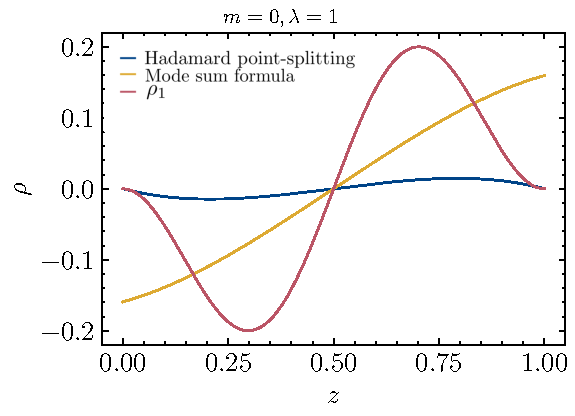
\includegraphics[width=0.45\textwidth]{Figures/dirichlet/hambjorn_annotated.pdf}
    \caption{Three different $\rho$ for the same massless scalar field subject to DBC: In blue, the correct prescription as explained in \cite{wernersson_vacuum_2021}. In orange, $\rho$ calculated through the mode sum \eqref{eq:mode-sum}. In red, $\rho$ defined through the mode sum formula, truncated to the first mode. }
    \label{fig:hambjorn}
\end{figure}
%\section{Computing the vacuum polarization}
\label{sec:Computing-the-vacuum-polarization}

To be able to compute Eq.~\eqref{eq:vacuum-polarization-long}, some rearrangements are to be done. By use of $-\omega_n = \omega_{-n}$, $\rho$ can be expressed as a single sum
\begin{align}
    \rho = \lim_{\tau \to 0} 
    \sum_{n>0}^{} 
        \left[ 
            (\omega_n - \varepsilon A_0) \lvert \phi_n\rvert^2 
            - (\omega_n + \varepsilon A_0) \lvert \phi_{-n}\rvert^2
        \right]e^{-i\omega_n \tau}
+ \frac{\varepsilon^2}{\pi} A_0 (z).
\end{align}
Although the limit and the sum do not commute (as one used to the mode sum formula might expect), if the coefficients of the sum decay fast enough, the limit and the sum indeed commute\marginnote{Who wrote this??}. After  commuting, the sum is cut off at some finite mode $N$, which induces oscillations of frequency $\Delta z = \frac{1}{N+1}$. These oscillations are an artifact of the cut off, which must be averaged out. 


\begin{figure}[t]
    \centering
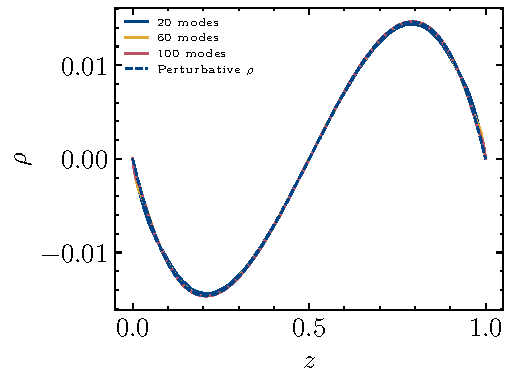
\includegraphics[width=0.8\textwidth]{Figures/dirichlet/unfilteredRhoaa.pdf}
    \caption{$\rho$ of the massless complex scalar field subject to a constant background electric field of strength $\lambda = 1$, for different mode cut-offs, as indicated in the legend. For reference, the perturbative vacuum polarization is given.}
    \label{fig:unfiilteredRhoaa}
\end{figure}
To achieve this, a low-pass filter is applied to the unfiltered vacuum polarization, by convoluting it with a normalized gaussian function, of approximately 3 oscillations of width. The $\rho$ resulting from the filtering is displayed in Fig.~\ref{fig:unfiilteredRhoaa}, where the filtering has been applied to the vacuum polarization resulting from different mode cut-offs (20, 60 and 100, as indicated by the legend). For reference, the vacuum polarization calculated from perturbative theory as per \cite{Wernersson:2020xeh} is also given.

\section{Convergence of the self-consistent fields}
\label{sec:convergence}


\begin{figure}[t]
    \begin{subfigure}{0.45\textwidth}
        \centering
        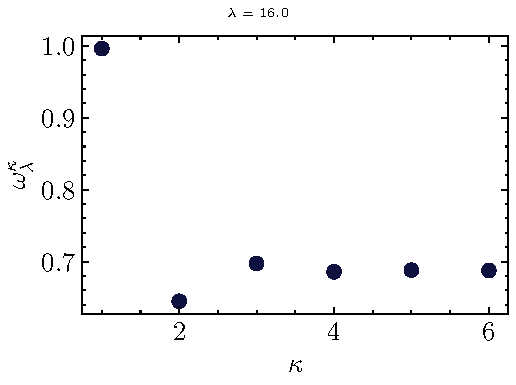
\includegraphics[width=\textwidth]{Figures/convergence/eigenvalues_lambda_16_dirichlet.pdf}
    \end{subfigure}
  \begin{subfigure}{0.45\textwidth}
        \centering
        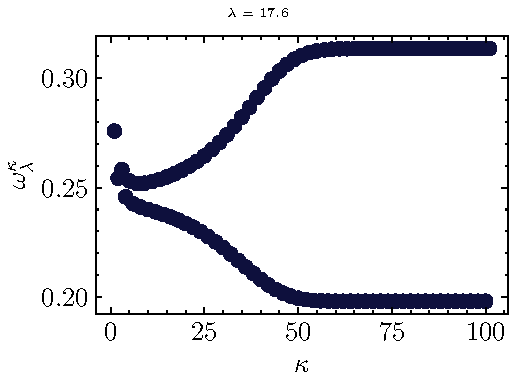
\includegraphics[width=\textwidth]{Figures/convergence/eigenvalues_lambda_17.599999999999998_dirichlet.pdf}
    \end{subfigure}
        \caption{$\omega_1$ of the massless scalar field with DBC for different values of $\lambda$ as a function of the iteration $\kappa$.}        \label{fig:convergence}

\end{figure}

The iterative procedure either
    converges,
    oscillates, or
    breaks down. 
    
The convergence of the iterative procedure described in Sec.~\ref{sec:The-iterative-procedure} is measured through the sequence $\{\omega_{1, \lambda}^\kappa\}_{\kappa>0}$. Examples of a converging sequence and an oscillating (non‑convergent) sequence are displayed in the top and bottom panels of Fig.~\ref{fig:convergence}, respectively. These cases can be understood from the perspective of fixed‑point theory, where we explicitly see whether the update function $f_{\lambda,c}$ is a contraction (top panel) or not (bottom panel).  We conjecture that one can always find a small enough $c$ such that the map $f_{\lambda,c   }$ is contracting.

The iterative procedure breaks down when complex $\omega$ appear. This happens if the candidate $\lambda +\Delta \lambda $ in the numerical continuation method is too far away from $\lambda$: the screening due to $\rho_\lambda$  is too weak compared to $A_{0, \lambda+\Delta \lambda}^1$, and the system effectively behaves as in the external field approximation with $\lambda>\lambda_c$.
The step $\Delta \lambda$ is reduced and the iterative procedure is tried again. 

% \begin{subfigure}{0.5\textwidth}
%     \centering
%     
\includegraphics[width=\textwidth]{subfigures/convergence/eigenvalues_lambda_12_dirichlet.pdf}
%     \caption{$\omega_1$ of the massless scalar field with DBC for $\lambda=12$ (weak-field regime) as a function of the iteration $\kappa.$  }
%     \label{fig:weak-field}
% \end{subfigure}

\bibliographystyle{abbrvnat}
\bibliography{main}

\end{document}
